%%%%%%%%%%%%%%%%%%%%%%%%%%%%%%%%%%%%%%%%%
% Short Sectioned Assignment
% LaTeX Template
% Version 1.0 (5/5/12)
%
% This template has been downloaded from:
% http://www.LaTeXTemplates.com
%
% Original author:
% Frits Wenneker (http://www.howtotex.com)
%
% License:
% CC BY-NC-SA 3.0 (http://creativecommons.org/licenses/by-nc-sa/3.0/)
%
%%%%%%%%%%%%%%%%%%%%%%%%%%%%%%%%%%%%%%%%%

%----------------------------------------------------------------------------------------
%	PACKAGES AND OTHER DOCUMENT CONFIGURATIONS
%----------------------------------------------------------------------------------------

\documentclass[paper=a4, fontsize=11pt]{scrartcl} % A4 paper and 11pt font size

\usepackage[T1]{fontenc} % Use 8-bit encoding that has 256 glyphs
\usepackage{fourier} % Use the Adobe Utopia font for the document - comment this line to return to the LaTeX default
\usepackage[english]{babel} % English language/hyphenation
\usepackage{amsmath,amsfonts,amsthm} % Math packages
\usepackage[utf8]{inputenc}
\usepackage{graphicx}
\usepackage{tabularx}
\usepackage{longtable}
\usepackage{threeparttable}
\usepackage{booktabs}
\usepackage{listings}
\usepackage[numbered,autolinebreaks,useliterate]{mcode}
\usepackage{float}
\usepackage{algpseudocode}

\usepackage{lipsum} % Used for inserting dummy 'Lorem ipsum' text into the template

\usepackage{sectsty} % Allows customizing section commands
\allsectionsfont{\centering \normalfont\scshape} % Make all sections centered, the default font and small caps

\usepackage{fancyhdr} % Custom headers and footers
\pagestyle{fancyplain} % Makes all pages in the document conform to the custom headers and footers
\fancyhead{} % No page header - if you want one, create it in the same way as the footers below
\fancyfoot[L]{} % Empty left footer
\fancyfoot[C]{} % Empty center footer
\fancyfoot[R]{\thepage} % Page numbering for right footer
\renewcommand{\headrulewidth}{0pt} % Remove header underlines
\renewcommand{\footrulewidth}{0pt} % Remove footer underlines
\setlength{\headheight}{13.6pt} % Customize the height of the header

\numberwithin{equation}{section} % Number equations within sections (i.e. 1.1, 1.2, 2.1, 2.2 instead of 1, 2, 3, 4)
\numberwithin{figure}{section} % Number figures within sections (i.e. 1.1, 1.2, 2.1, 2.2 instead of 1, 2, 3, 4)
\numberwithin{table}{section} % Number tables within sections (i.e. 1.1, 1.2, 2.1, 2.2 instead of 1, 2, 3, 4)

\setlength\parindent{0pt} % Removes all indentation from paragraphs - comment this line for an assignment with lots of text

%----------------------------------------------------------------------------------------
%	TITLE SECTION
%----------------------------------------------------------------------------------------

\newcommand{\horrule}[1]{\rule{\linewidth}{#1}} % Create horizontal rule command with 1 argument of height

\title{	
\normalfont \normalsize 
\textsc{Faculdade de Engenharia da Universidade do Porto} \\ [25pt] % Your university, school and/or department name(s)
\horrule{0.5pt} \\[0.4cm] % Thin top horizontal rule
\LARGE Machnine Learning (PDEEC0049 : 15-782PP)\\ \Large Homework 1 \\ % The assignment title
\horrule{2pt} \\[0.5cm] % Thick bottom horizontal rule
}

\author{António Damião das Neves Rodrigues (200400437 : 700098386)} % Your name

\date{\normalsize\today} % Today's date or a custom date

\begin{document}

\maketitle % Print the title

\section{Problem 1}

Following the definition of the conditional expectation of a random variable $L$,
given the event $L > n$ with $P(L > n) > 0$, we get:

\begin{equation}
    \textbf{E}\left[L|L > n\right] = \sum\limits_{l} l \thinspace P(L|L > n)
    \label{eq:1-1-definition}
\end{equation}

Applying Bayes' theorem to~\ref{eq:1-1-definition} we get:

\begin{equation}
    \textbf{E}\left[L|L > n\right] = \sum\limits_{l} l \thinspace P(L|L > n) = \sum\limits_{l} l \thinspace \frac{P(L > n|L)P(L)}{P(L > n)}, \quad P(L > n) > 0
    \label{eq:1-1-bayes}
\end{equation}

The distribution of $P(L > n|L)$ can be easily determined by recognizing that if 
we are given a particular $L=l$, $L$ is either larger than $n$ 
or not larger than $n$, i.e.:

\begin{equation}
    P(L > n|L = l) = \left\{ 
        \begin{array}{rl}
            1 &\mbox{ \text{if $l > n$}} \\
            0 &\mbox{ \text{if $l \le n$}}
        \end{array} \right.
    \label{eq:1-1-larger}
\end{equation}

Applying~\ref{eq:1-1-larger} in the expression for 
\textbf{E}$\left[L|L > n\right]$ (\ref{eq:1-1-bayes}), we get:

\begin{equation}
    \textbf{E}\left[L|L > n\right] = \sum\limits_{l} l \thinspace \frac{P(L > n|L)P(L)}{P(L > n)} = \sum\limits_{l > n} l \thinspace \frac{P(L)}{P(L > n)}, \quad P(L > n) > 0
    \label{eq:1-1-bayes-2}
\end{equation}

Considering $L = [l_{min}, l_{min + 1}, ... , n - 1, n, n + 1, ... , l_{max - 1}, 
l_{max}]$ where $l_{min} < l_{min + 1} < ... < n - 1 < n < n + 1 < ... < 
l_{max - 1} < l_{max}$, we can express \textbf{E}$\left[L|L > n\right]$ in 
the form shown in~\ref{eq:1-1-bayes-3}:

\begin{equation}
\begin{split}
    \textbf{E}\left[L|L > n\right] &= \sum\limits_{l > n} l \thinspace \frac{P(L)}{P(L > n)}\\ 
    &= \frac{(n+1)P(L = n+1) + (n+2)P(L = (n+2)) + ... + l_{max}P(L = l_{max})}{P(L = (n+1)) + P(L = (n+2)) + ... + P(L = l_{max})}, \quad P(L > n) > 0
    \label{eq:1-1-bayes-3}
\end{split}
\end{equation}

So \textbf{E}$\left[L|L > n\right]$ produces a mean for values of $L$ 
within the interval $\left]n, l_{max}\right]$. If $P(L > n) > 0$, then 
\textbf{E}$\left[L|L > n\right] \in 
\left]n, l_{max}\right]$.\\ 

The addition an element $l = (n - 1) < n$ will contribute to lower the value of 
the average, i.e. \textbf{E}$\left[L|L > n - 1\right] < \textbf{E}\left[L|L > 
n\right]$. The reduction of the value of the average occurs for every $l' < n$, 
such that $l' \geq l_{min}$, i.e. \textbf{E}$\left[L|L > l'\right] < \textbf{E}\left[L|L > 
n\right]$, with $l_{min} \le l' < n$. We can consider 
\textbf{E}$\left[L\right]$ as \textbf{E}$\left[L|L > l'\right]$, when 
$l' \to l_{min}$.\\ 

Therefore \textbf{E}$\left[L\right] =  \textbf{E}\left[L|L > l' \to l_{min} \right] < \textbf{E}\left[L|L > n\right]$.\\

Looking at expression~\ref{eq:1-1-bayes-3}, if we consider the case in which 
$n \to l_{min}$, i.e. as $P(L > n) \to 1$ (and consequently $P(L \le n) \to 0$), 
it can be seen that \textbf{E}$\left[L|L > n\right] \to \textbf{E}\left[L\right]$. 
Hence, here is why the inequality is strict for $P(L \le n) > 0$.

\section{Problem 2}

\subsection{}

Figure~\ref{fig:2-1} depicts the scatter plots of the observations for each one 
of the sets $X_1$, $X_2$ and $X_3$ over the two-dimensional space $(x_1,x_2)$.

\begin{figure}[H]

    \centering
    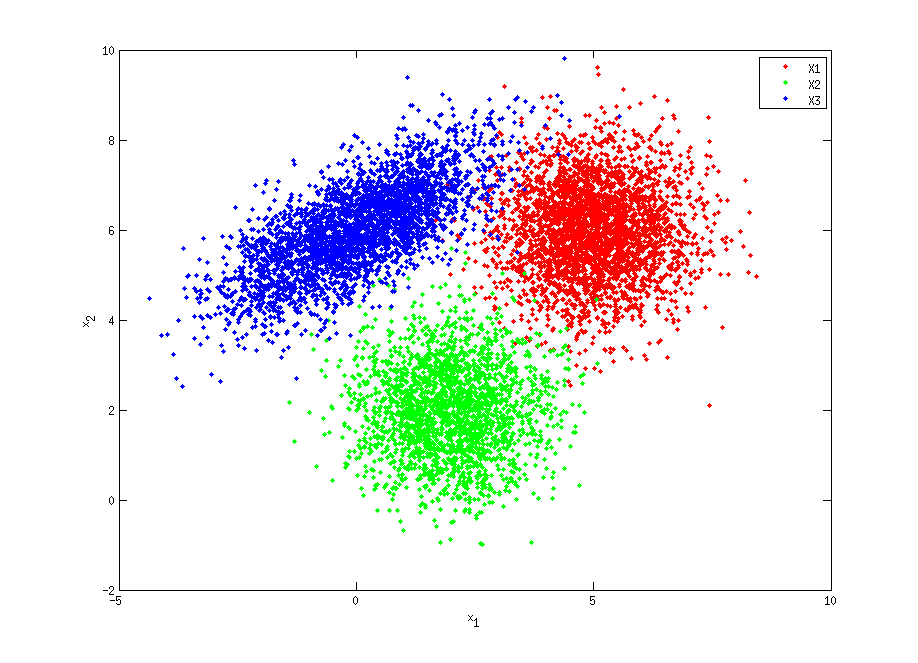
\includegraphics[width=0.85\textwidth]{figures/2-1.png}
    \caption{Graphical representation of the problem training set, consisting 
            in three groups of observations $X_1$, $X_2$ and $X_3$.}
    \label{fig:2-1}

\end{figure}

\subsection{}
\label{subsec:2-2}

The values of $\mu$ and $\sum$ (covariance matrix) for each one of the 
distributions of the observation sets $X_1$, $X_2$ and $X_3$ (obtained via 
MATLAB commands \verb%mean% and \verb%cov%) are shown in Table~\ref{tab:2-2}.\\

\begin{table}[H]
\begin{center}
    \begin{threeparttable}
    \small
        \begin{tabularx}{0.60\textwidth}{ c | c | c  }
            %\hline
            \textbf{Observation Set}    & \boldmath$\mu$ & \boldmath$\sum$\\ [0.5ex]
            \hline 
            & & \\ [0.0ex]
            ${X}_{1}$   & $\begin{bmatrix}  5.0029 & 5.9756 \end{bmatrix}$ & $\begin{bmatrix} 1.0161 & 0.0135 \\ 0.0135 & 1.0157 \end{bmatrix}$\\ [0.5ex]
            %\hline
            & & \\ [0.0ex]
            ${X}_{2}$   & $\begin{bmatrix}  1.9830 & 2.0029 \end{bmatrix}$ & $\begin{bmatrix} 1.0183 & 0.0044 \\ 0.0044 & 1.0072 \end{bmatrix}$\\ [0.5ex]
            %\hline
            & & \\ [0.0ex]
            ${X}_{3}$   & $\begin{bmatrix}  0.0154 & 6.0173 \end{bmatrix}$ & $\begin{bmatrix} 1.9229 & 0.9801 \\ 0.9801 & 0.9882 \end{bmatrix}$\\ [0.5ex]
            %\hline
            %\hline
        \end{tabularx}

    \caption{Values of $\mu$ and $\sum$ for each one of the distributions 
        relative to the sets of observations $X_1$, $X_2$ and $X_3$.}
    \label{tab:2-2}
    \end{threeparttable}
    \end{center}
\end{table}

By combined inspection of Figure~\ref{fig:2-1} and Table~\ref{tab:2-2}, one can 
verify that the values of $\mu$ on the table are close to the centers of the 
respective `swarms' of observations in the figure.\\

With $\mu$ and $\sum$ estimated from the data, we can now find 
the expressions for each of the models $N(\text{x}|\mu_i,\sum\text{$_{i}$})$:

\begin{equation}
        N(\text{x}|\mu_i,\sum\text{$_{i}$}) = \frac{e^{-\frac{1}{2}\left[\left(\text{x} - \mu_{i}\right)\textsuperscript{T}{\sum\text{$^{-1}_{i}$}}\left(\text{x} - \mu_{i}\right)\right]}}{2\pi{\left|\sum\text{$_{i}$}\right|}^{\frac{1}{2}}}
    \label{eq:normal-u12-1}
\end{equation}

These are models for the class-conditional distributions for each class 
$C_i$, i.e. each provides the value of the probability for \textbf{x}, given 
that the class is $C_i$. Therefore:

\begin{equation}
        p(\text{x}|C_i) = \frac{e^{-\frac{1}{2}\left[\left(\text{x} - \mu_{i}\right)\textsuperscript{T}{\sum\text{$^{-1}_{i}$}}\left(\text{x} - \mu_{i}\right)\right]}}{2\pi{\left|\sum\text{$_{i}$}\right|}^{\frac{1}{2}}}
    \label{eq:normal-u12-1}
\end{equation}

\subsection{}
\label{subsec:2-3}

With the expressions for the class-conditional distributions, we can now apply
Bayes' theorem (as given in (1.82) in~\cite{Bishop2006}) to find the posterior 
probabilities $p(C_i|\text{x})$:

\begin{equation}
    p(C_i|\text{x}) = \frac{p(\text{x}|C_i)p(C_i)}{p(\text{x})}
    \label{eq:posteriors}
\end{equation}

The prior probabilities $p(C_i)$, can inferred by 
considering the number of observations in each training set $N_{X_i}$, 
divided by the total number of points in the three training sets $N = N_{X_i} 
+ N_{X_j} + N_{X_k}$:

\begin{equation}
    p(C_i) = \frac{N_{X_i}}{N_{X_i} + N_{X_j} + N_{X_k}} = \frac{N_{X_i}}{N}
    \label{eq:priors}
\end{equation}

The boundary between classes $C_i$ and $C_k$ can be found by determining the 
common points between $p(C_i|\text{x})$ and 
$p(C_k|\text{x})$, i.e.:

\begin{equation}
\begin{split}
        \frac{p(\text{x}|C_i)p(C_i)}{p(\text{x})} &= \frac{p(\text{x}|C_j)p(C_j)}{p(\text{x})}\\
        \frac{p(C_i)e^{-\frac{1}{2}\left[\left(\text{x} - \mu_{i}\right)\textsuperscript{T}{\sum\text{$^{-1}_{i}$}}\left(\text{x} - \mu_{i}\right)\right]}}{2\pi{\left|\sum\text{$_{i}$}\right|}^{\frac{1}{2}}} &= \frac{p(C_j)e^{-\frac{1}{2}\left[\left(\text{x} - \mu_{j}\right)\textsuperscript{T}{\sum\text{$^{-1}_{j}$}}\left(\text{x} - \mu_{j}\right)\right]}}{2\pi{|\sum\text{$_{j}$}|}^{\frac{1}{2}}}\\
        \frac{e^{-\frac{1}{2}\left[\left(\text{x} - \mu_{i}\right)\textsuperscript{T}{\sum\text{$^{-1}_{i}$}}\left(\text{x} - \mu_{i}\right)\right]}}{e^{-\frac{1}{2}\left[\left(\text{x} - \mu_{j}\right)\textsuperscript{T}{\sum\text{$^{-1}_{j}$}}\left(\text{x} - \mu_{j}\right)\right]}} &= \frac{{p(C_j)\left|\sum\text{$_{i}$}\right|}^{\frac{1}{2}}}{{p(C_i)|\sum\text{$_{j}$}|}^{\frac{1}{2}}}\\
        e^{-\frac{1}{2}\left[\left(\text{x} - \mu_{i}\right)\textsuperscript{T}{\sum\text{$^{-1}_{i}$}}\left(\text{x} - \mu_{i}\right)
        - \left(\text{x} - \mu_{j}\right)\textsuperscript{T}{\sum\text{$^{-1}_{j}$}}\left(\text{x} - \mu_{j}\right)\right]} &= e^{\ln{\left(\frac{{p(C_j)\left|\sum\text{$_{i}$}\right|}^{\frac{1}{2}}}{{p(C_i)|\sum\text{$_{j}$}|}^{\frac{1}{2}}}\right)}}
    \label{eq:gauss-exp}
\end{split}
\end{equation}

Both sides of equation~\ref{eq:gauss-exp} are equal when the exponents are the 
same. By evaluating the exponents only, we get equation~\ref{eq:exponents-1}:

\begin{equation}
        -\frac{1}{2}\left[\left(\text{x} - \mu_{i}\right)\textsuperscript{T}{\sum\text{$^{-1}_{i}$}}\left(\text{x} - \mu_{i}\right)
        - \left(\text{x} - \mu_{j}\right)\textsuperscript{T}{\sum\text{$^{-1}_{j}$}}\left(\text{x} - \mu_{j}\right)\right] - \ln{\left(\frac{{p(C_j)\left|\sum\text{$_{i}$}\right|}^{\frac{1}{2}}}{{p(C_i)\left|\sum\text{$_{j}$}\right|}^{\frac{1}{2}}}\right)} = 0
        %-\frac{1}{2}\left(\begin{bmatrix} x_1 \\ x_2 \end{bmatrix} - \begin{bmatrix} 5.0029 \\ 5.9756 \end{bmatrix}\right)^{\text{T}}
        %\begin{bmatrix} 0.9844 & -0.0131 \\ -0.0131 & 0.9848 \end{bmatrix}
        %\left(\begin{bmatrix} x_1 \\ x_2 \end{bmatrix} - \begin{bmatrix} 5.0029 \\ 5.9756 \end{bmatrix}\right) = 0
    \label{eq:exponents-1}
\end{equation}

For the boundary \textbf{u\textsubscript{ij}} between classes {\boldmath$C_i$} and 
{\boldmath$C_j$}, we therefore have expression~\ref{eq:exponents-1}, which is 
a curve on two-dimensional space $(x_1,x_2)$. Boundaries 
\textbf{u\textsubscript{12}}, \textbf{u\textsubscript{13}} and 
\textbf{u\textsubscript{23}} are given by expressions~\ref{eq:boundary-u12-1},
~\ref{eq:boundary-u13-1} and~\ref{eq:boundary-u23-1} respectively:
%\begin{equation}
%        -\frac{1}{2}\left[\left(\text{x} - \mu_{X_1}\right)\textsuperscript{T}{\sum\text{$^{-1}_{X_1}$}}\left(\text{x} - \mu_{X_1}\right)
%        - \left(\text{x} - \mu_{X_2}\right)\textsuperscript{T}{\sum\text{$^{-1}_{X_2}$}}\left(\text{x} - \mu_{X_2}\right)\right] - \ln{\left(\frac{{\left|\sum\text{$_{X_2}$}%\right|}^{\frac{1}{2}}}{{\left|\sum\text{$_{X_1}$}\right|}^{\frac{1}{2}}}\right)} = 0
        %-\frac{1}{2}\left(\begin{bmatrix} x_1 \\ x_2 \end{bmatrix} - \begin{bmatrix} 5.0029 \\ 5.9756 \end{bmatrix}\right)^{\text{T}}
        %\begin{bmatrix} 0.9844 & -0.0131 \\ -0.0131 & 0.9848 \end{bmatrix}
        %\left(\begin{bmatrix} x_1 \\ x_2 \end{bmatrix} - \begin{bmatrix} 5.0029 \\ 5.9756 \end{bmatrix}\right) = 0
%    \label{eq:boundary-u12-1}
%\end{equation}

%Expressing~\ref{eq:boundary-u12-1} in terms of $x_1$ and $x_2$, we 
%get expression~\ref{eq:boundary-u12-2}:

\begin{equation}
        -\frac{1}{2}\left[\left(\text{x} - \mu_{1}\right)\textsuperscript{T}{\sum\text{$^{-1}_{1}$}}\left(\text{x} - \mu_{1}\right)
        - \left(\text{x} - \mu_{2}\right)\textsuperscript{T}{\sum\text{$^{-1}_{2}$}}\left(\text{x} - \mu_{2}\right)\right] - \ln{\left(0.7\frac{{\left|\sum\text{$_{1}$}\right|}^{\frac{1}{2}}}{{\left|\sum\text{$_{2}$}\right|}^{\frac{1}{2}}}\right)} = 0
    \label{eq:boundary-u12-1}
\end{equation}

\begin{equation}
        -\frac{1}{2}\left[\left(\text{x} - \mu_{1}\right)\textsuperscript{T}{\sum\text{$^{-1}_{1}$}}\left(\text{x} - \mu_{1}\right)
        - \left(\text{x} - \mu_{3}\right)\textsuperscript{T}{\sum\text{$^{-1}_{3}$}}\left(\text{x} - \mu_{3}\right)\right] - \ln{\left(\frac{{\left|\sum\text{$_{1}$}\right|}^{\frac{1}{2}}}{{\left|\sum\text{$_{3}$}\right|}^{\frac{1}{2}}}\right)} = 0
    \label{eq:boundary-u13-1}
\end{equation}

\begin{equation}
        -\frac{1}{2}\left[\left(\text{x} - \mu_{2}\right)\textsuperscript{T}{\sum\text{$^{-1}_{2}$}}\left(\text{x} - \mu_{2}\right)
        - \left(\text{x} - \mu_{3}\right)\textsuperscript{T}{\sum\text{$^{-1}_{3}$}}\left(\text{x} - \mu_{3}\right)\right] - \ln{\left(1.4\frac{{\left|\sum\text{$_{2}$}\right|}^{\frac{1}{2}}}{{\left|\sum\text{$_{3}$}\right|}^{\frac{1}{2}}}\right)} = 0
    \label{eq:boundary-u23-1}
\end{equation}

Let $f_{ij}(x)$ be the left side of equations~\ref{eq:boundary-u12-1},
~\ref{eq:boundary-u13-1} and~\ref{eq:boundary-u23-1}. For every class pair 
evaluation, given an observation $x$, we should decide for class $C_i$ if $f_{ij}(x) \geq 0$ or class 
$C_j$ if $f_{ij}(x) < 0$. Note that each $f_{ij}(x)$ determines if an 
observation $x$ belongs to class $C_i$, considering the border with class 
$C_j$. In order to completely determine the class for $x$, we must evaluate the 
remaining border via $f_{ik}(x)$ or $f_{jk}(x)$.\\

One strategy to follow in order to assign an observation $x$ to a class $C_1$, 
$C_2$ or $C_3$ can be as shown below. Note that for $N = 3$ classes the 
proposed nested set of conditional statements is feasible, however such an 
approach might get too complex for a larger $N$.\\

\begin{algorithmic}
\ForAll{observation $x$} 

\If {$f_{12}(x) \geq 0$}

    \If {$f_{31}(x) \geq 0$}
        \State assign observation $x$ to class $C_3$
    \Else
        \State assign observation $x$ to class $C_1$
    \EndIf

\ElsIf {$f_{23}(x) \geq 0$} 
    \State assign observation $x$ to class $C_2$
\Else 
    \State assign observation $x$ to class $C_3$
\EndIf

\EndFor
\end{algorithmic}

\subsection{}

Listings~\ref{lst:2-4-classifier-code} and~\ref{lst:2-4-classifier-code-dscrmnt} 
provide the MATLAB code used for classifying the observation set $X_x$. The 
results are graphically shown in Figure~\ref{fig:2-4-classifier} (same color 
code as in Figure~\ref{fig:2-1}). The class boundaries obtained 
in~\ref{subsec:2-3} are also plotted. (using MATLAB command \verb=ezplot()=).

\begin{lstlisting}[label=lst:2-4-classifier-code,caption={MATLAB code for 2.4.}]
clear

% load the problem's data
load('.../trainingset.mat');

% total number of observations from the training sets
N = length(X1(:,1)) + length(X2(:,1)) + length(X3(:,1));

% calculate the parameters for each one of the distributions Xk, to be 
% used in the discriminant functions dscrmnt(x, ...)

% mean
U1 = mean(X1);

% covariance matrix
Cov1 = cov(X1);

% inverse of the covariance matrix (let's calculate it beforehand and not 
% every time dsrmnt(x, ...) is ran)
iCov1 = inv(Cov1);

% the factor which affects the Gaussian distributions of Xk, including 
% the prior probability for each class, pri
pr1 = length(X1(:,1))/(N);
k1 = pr1/(2*pi*sqrt(det(Cov1)));

U2 = mean(X2);
Cov2 = cov(X2);
iCov2 = inv(Cov2);
pr2 = length(X2(:,1))/(N);
k2 = pr2/(2*pi*sqrt(det(Cov2)));

U3 = mean(X3);
Cov3 = cov(X3);
iCov3 = inv(Cov3);
pr3 = length(X3(:,1))/(N);
k3 = pr3/(2*pi*sqrt(det(Cov3)));

% for convenience, create arrays to accomodate the each observation 
% belonging to class Ck
C1 = [];
C2 = [];
C3 = [];


figure;
hold on;

[r,c] = size(XX);

% for each observation x in XX, determine its class Ck following the 
% heuristics defined in 2.3 b)
for i=1:r

    x = XX(i,:);
    
    % descriminant function template for C1 and C2
    if dscrmnt(x,U1,U2,iCov1,iCov2,log(k2/k1)) == 1
        
        % use the descriminant function template for C3 and C1, to 
        % evaluate the boundary u13
        if dscrmnt(x,U3,U1,iCov3,iCov1,log(k1/k3)) == 1
            
            % have found an observation which falls into C3
            % add an entry to the appropriate class array
            C3 = [C3; x];
            
        else
            
            % x indeed belongs to C1
            C1 = [C1; x];
        
        end
    
    % descriminant function template for C2 and C3
    elseif dscrmnt(x,U2,U3,iCov2,iCov3,log(k3/k2)) == 1
        
        % x indeed belongs to C1
        C2 = [C2; x];
        
    else
        
        % x belongs to C3
        C3 = [C3; x];

    end
    
end

% print the axis labels
xlabel('x_1');
ylabel('x_2');

% plot the observations in Xx, the color indicates the class to which an 
% observation was assigned (same color code as in 2.1)
plot(C1(:,1), C1(:,2), 'r.');
plot(C2(:,1), C2(:,2), 'g.');
plot(C3(:,1), C3(:,2), 'b.');

% let's plot the class boundaries
syms x1 x2
u12=-0.5*(([x1 x2] - U1)*iCov1*([x1; x2]-U1') - ([x1 x2] - U2)*iCov2*([x1; x2]-U2')) - log(k2/k1);
u13=-0.5*(([x1 x2] - U1)*iCov1*([x1; x2]-U1') - ([x1 x2] - U3)*iCov3*([x1; x2]-U3')) - log(k3/k1);
u23=-0.5*(([x1 x2] - U2)*iCov2*([x1; x2]-U2') - ([x1 x2] - U3)*iCov3*([x1; x2]-U3')) - log(k3/k2);

pu12 = ezplot(u12,[2,8,-2,6]);
h = get(gca,'children');
set(h(1),'linestyle','-.','color','b','linewidth',1);

pu13 = ezplot(u13,[2,5,4,12]);
h = get(gca,'children');
set(h(1),'linestyle','-.','color','g','linewidth',1);

pu23 = ezplot(u23,[-3,2,-2,6]);
h = get(gca,'children');
set(h(1),'linestyle','-.','color','r','linewidth',1);

% color code for the observation-class assignment
legend('C_1','C_2','C_3','u12','u13','u23');
\end{lstlisting}

\begin{lstlisting}[label=lst:2-4-classifier-code-dscrmnt,caption={MATLAB code for 2.4.}]
% template for the discriminant function between class a vs. class b.
% returns 1 if x is classified as belonging to class 'a', 0 if 'b'.

% classes a and b which are discriminated by dscrmnt() are determined by 
% setting the appropriate input parameters Uk, iCovk and C. 

% e.g. the discriminant function between classes 1 and 2 is 
% dscrmnt(x,U1,U2,iCov1,iCov2,C12).
function [dscrmnt] = dscrmnt(x,Ua,Ub,iCova,iCovb,C)

if (-0.5*((x-Ua)*iCova*(x-Ua)' - (x-Ub)*iCovb*(x-Ub)') - C) >= 0
    
    dscrmnt = 1;

else
    
    dscrmnt = 0;

end
\end{lstlisting}

\begin{figure}[H]

    \centering
    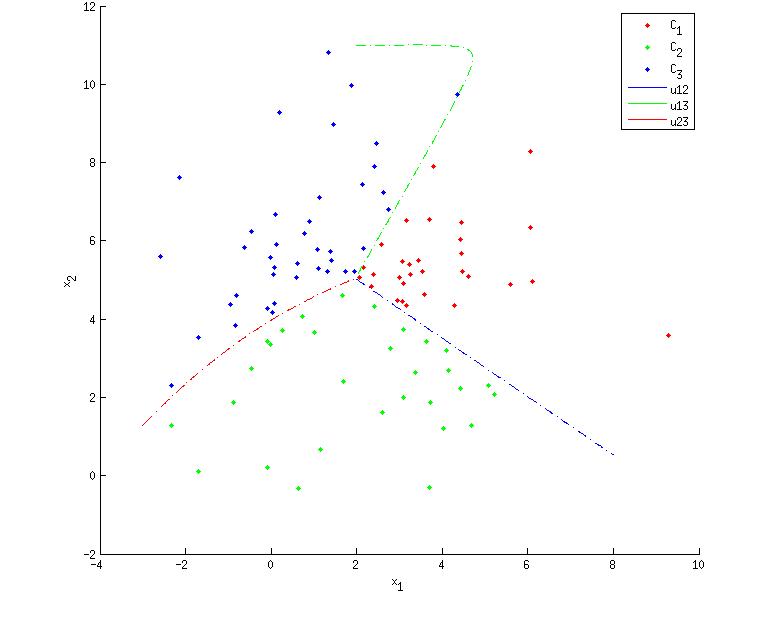
\includegraphics[width=0.85\textwidth]{figures/2-4.png}
    \caption{Graphical representation of the classification of the observations 
            in set $X_x$. The class boundaries obtained in~\ref{subsec:2-3} are 
            also plotted.}
    \label{fig:2-4-classifier}

\end{figure}

\subsection{}

The exercise asks for way to calculate the probability of a selected class 
given an observation, i.e. the posterior probability $p(C_i|x)$. This 
probability can be found by using Bayes' theorem (as given in (1.82) 
in~\cite{Bishop2006}):

\begin{equation}
    p(C_i|\textbf{x}) = \frac{p(\textbf{x}|C_i)p(C_i)}{p(\textbf{x})} = \frac{p(\textbf{x}|C_i)p(C_i)}{\sum\limits_{i} p(\textbf{x}|C_i) p(C_i)}
    \label{eq:posterior}
\end{equation}

The class-conditional probabilities for each class $C_i$ are obtained via the 
estimations performed in Section~\ref{subsec:2-2}.\\

The prior probabilities $p(C_i)$, can be inferred as indicated in Section~\ref{subsec:2-3}, i.e. by 
considering the number of observations in each training set $N_{X_i}$, 
divided by the total number of points in the three training sets $N = N_{X_i} 
+ N_{X_j} + N_{X_k}$:

\begin{equation}
    p(C_i) = \frac{N_{X_i}}{N_{X_i} + N_{X_j} + N_{X_k}} = \frac{N_{X_i}}{N}
    \label{eq:prior}
\end{equation}

With the class-conditional and prior probabilities determined, Bayes' theorem 
should be used to find $p(C_k|x)$.\\

\section{Problem 3}

This is a classification problem for two classes $C_A$ and $C_B$, and a random 
variable \textbf{$x$} , with part of the inference stage parameters 
already determined: the class-conditional densities $p(x|C_A)$ and $p(x|C_B)$, 
as well as the prior class probabilities $p(C_A)$ and $p(C_B)$. Therefore, 
approach (a) given in Section 1.5.4 of~\cite{Bishop2006} is appropriate to 
tackle this problem.

\subsection{}
\label{subsec:3-1}

With part of the inference stage out of the way, one should now use Bayes' 
theorem to determine the posterior class probabilities $p(C_A|x)$ and 
$p(C_B|x)$, which will allow us to go ahead into the decision phase. 
Applying Bayes' theorem (as given in (1.82) in~\cite{Bishop2006}), we get:

\begin{equation}
    p(C_A|x) = \frac{p(x|C_A) p(C_A)}{p(x)} = \frac{\text{0.4}e^{-x}}{p(x)}, \quad x \geq 0
    \label{eq:cond-a}
\end{equation}

\begin{equation}
    p(C_B|x) = \frac{p(x|C_B) p(C_B)}{p(x)} = \frac{\frac{\text{0.6}}{\sqrt{2\pi}}e^{-(x-2)^2}}{p(x)}, \quad x \geq 0
    \label{eq:cond-b}
\end{equation}

From the combination of the sum and product rules of probability (see (1.10) and 
(1.11) in~\cite{Bishop2006}) and using the given expressions for the conditional 
and prior probabilities, we get the following expression for $p(x)$:

\begin{equation}
    p(x) = \sum\limits_{k} p(x|C_k) p(C_k) = \text{0.4}e^{-x} + \frac{\text{0.6}}{\sqrt{2\pi}}e^{-(x-2)^2}, \quad x \geq 0
    \label{eq:prod-rule}
\end{equation}

Applying~\ref{eq:prod-rule} in equations~\ref{eq:cond-a} and \ref{eq:cond-b}, 
we get the final expressions for $p(C_A|x)$ and $p(C_B|x)$:

\begin{equation}
    p(C_A|x) = \frac{\text{0.4}e^{-x}}{\text{0.4}e^{-x} + \frac{\text{0.6}}{\sqrt{2\pi}}e^{-(x-2)^2}}, \quad x \geq 0
    \label{eq:cond-a-final}
\end{equation}

\begin{equation}
    p(C_B|x) = \frac{\frac{\text{0.6}}{\sqrt{2\pi}}e^{-(x-2)^2}}{\text{0.4}e^{-x} + \frac{\text{0.6}}{\sqrt{2\pi}}e^{-(x-2)^2}}, \quad x \geq 0
    \label{eq:cond-b-final}
\end{equation}

With the posterior probabilities $p(C_A|x)$ and $p(C_B|x)$, we can now 
determine the decision boundaries $\hat{x}$ and consequently the decision regions 
$\mathcal{R}$ which minimize the misclassification rate. In this case, the same 
reasoning as that used in Section 1.5.1 of~\cite{Bishop2006} can be applied, 
i.e. in order to minimize the misclassification rate, each value of $x$ 
should be assigned to the class for which the probability $p(C_k|x)$ is the 
largest.\\ 

We should then find the values of $x$ for which 
$p(C_k|x)$ intersect in order to determine the $N$ decision boundaries 
$\hat{x}_n$ and then evaluate which posterior probability $p(C_k|x)$ has the 
highest value along each one of the $N+1$ resulting decision regions 
$\mathcal{R}_n$:

\begin{equation}
\begin{split}
    p(C_A|x) & = p(C_B|x) \\
    \text{0.4}e^{-x} & = \frac{\text{0.6}}{\sqrt{2\pi}}e^{-(x-2)^2} \\
    \frac{e^{-x}}{e^{-(x-2)^2}} & = e^{\ln\left(\frac{\text{3}}{2\sqrt{2\pi}}\right)} \\
    e^{x^2-5x+4} & = e^{\ln\left(\frac{\text{3}}{2\sqrt{2\pi}}\right)}, \quad x \geq 0
    %\Leftrightarrow  x^2 -5x + \left(4 - \ln\left(\frac{\text{3}}{2\sqrt{2\pi}}\right)\right) & = 0, \quad x \geq 0
    \label{eq:intersect-1}
\end{split}
\end{equation}

Both sides of equation~\ref{eq:intersect-1} are equal when the exponents are the 
same. By evaluating the exponents only, we get equation~\ref{eq:intersect-2}:

\begin{equation}
    x^2-5x+\left(4 - \ln\left(\frac{\text{3}}{2\sqrt{2\pi}}\right)\right) = 0, \quad x \geq 0
    \label{eq:intersect-2}
\end{equation}

Solving~\ref{eq:intersect-2} one gets the following two values of $x$ for the 
boundaries, $\hat{x}_{1}$ and $\hat{x}_{2}$:

\[ \hat{x}_{1} = \frac{5 - \sqrt{25 - 4\left(4 - \ln\left(\frac{\text{3}}{2\sqrt{2\pi}}\right)\right)}}{2} \approx 1.1822 
    \quad \quad \hat{x}_{2} = \frac{5 + \sqrt{25 - 4\left(4 - \ln\left(\frac{\text{3}}{2\sqrt{2\pi}}\right)\right)}}{2} \approx 3.8178 \] 

We therefore have three regions: $\mathcal{R}_{1}$, $\mathcal{R}_{2}$ and 
$\mathcal{R}_{3}$, separated by boundaries $\hat{x}_{1}$ and $\hat{x}_{2}$ 
respectively. Evaluating the values of $p(C_k|x)$ in the vicinities of both 
$\hat{x}_{1}$ and $\hat{x}_{2}$, one gets the decision regions given in 
Table~\ref{tab:3-1-class-ass}.\\

\begin{table}[H]
\begin{center}
    \begin{threeparttable}
    \small
        \begin{tabularx}{0.60\textwidth}{ X | X | X  }
            %\hline
            \textbf{Region}     & \textbf{Class} & \textbf{Interval\tnote{1}}\\ [0.5ex]
            \hline
            $\mathcal{R}_{1}$   & $C_A$ & $ 0 \le x < \hat{x}_1$ \\ [0.5ex]
            %\hline
            $\mathcal{R}_{2}$   & $C_B$ & $ \hat{x}_1 \le x < \hat{x}_2$\\ [0.5ex]
            %\hline
            $\mathcal{R}_{3}$   & $C_A$ & $ \hat{x}_2 \le x < +\infty$\\ [0.5ex]
            %\hline
            %\hline
        \end{tabularx}

        \begin{tablenotes}
            \footnotesize
            \item[1]The inclusions\slash exclusions of points $x = \hat{x}_1$ 
            and $x = \hat{x}_2$ into\slash from each one of the regions was 
            arbitrary.
        \end{tablenotes}
    \caption{Decision regions of the Bayes classifier.}
    \label{tab:3-1-class-ass}
    \end{threeparttable}
    \end{center}
\end{table}

Figure~\ref{fig:3-1} provides a graphical representation of the proposed 
solution, including decision boundaries and probability 
density functions.

\begin{figure}[H]

    \centering
    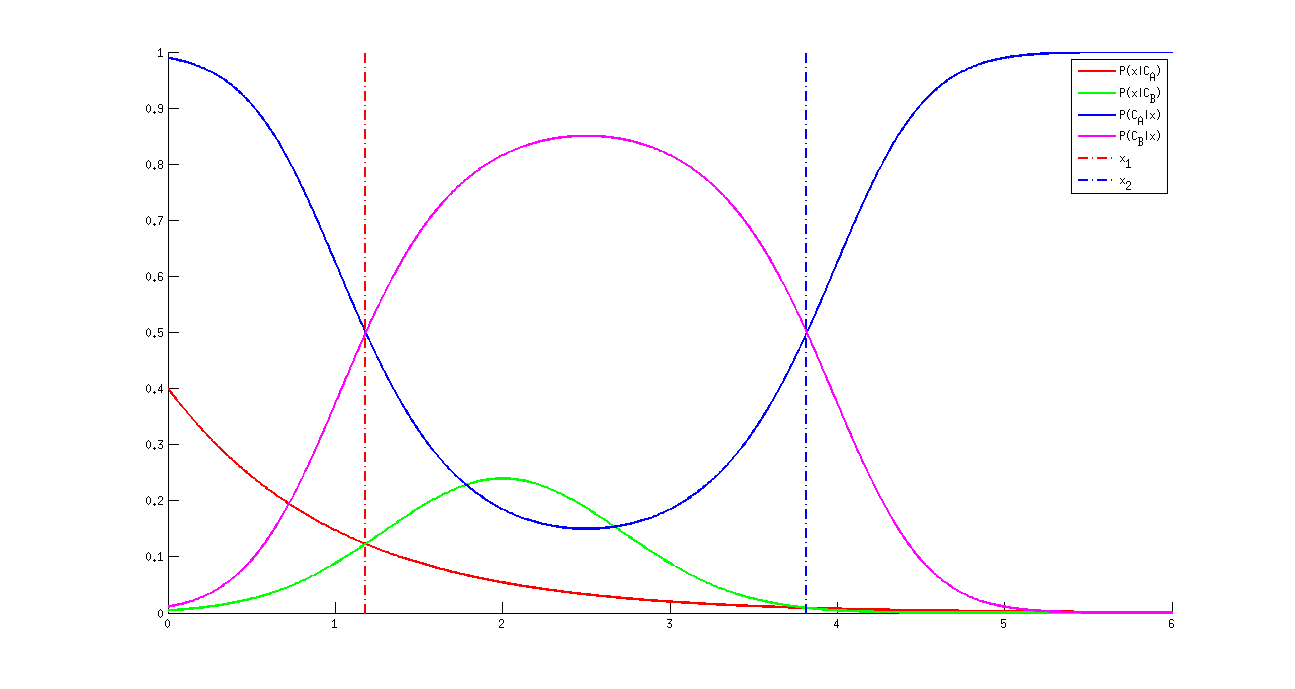
\includegraphics[width=1.00\textwidth]{figures/3-1.png}
    \caption{Graphical representation of the proposed 
solution, including decision boundaries and probability 
density functions.}
    \label{fig:3-1}

\end{figure}

\subsection{}
\label{subsec:3-2}

Considering $x = 1$, since $x \le \hat{x}_1$, it lies in decision region 
$\mathcal{R}_{1}$, therefore the predicted class for this observation is 
$C_A$. The probability of error can be determined by the value of the posterior 
probability for class $C_B$ given $x = 1$, $p(C_B|x = 1)$. Applying $x = 1$ 
in~\ref{eq:cond-b-final}, we get $p(C_B|x = 1) \approx 0.3744$.

\subsection{}

We define the loss matrix $L$ as shown below (each element $L_{kj}$ is the 
penalty value for assigning an observation $x$ to class $C_j$ although it 
belongs to $C_k$):

\begin{equation}
    L = \begin{bmatrix} L_{AA} & L_{AB} \\ L_{BA} & L_{BB} \end{bmatrix} = \begin{bmatrix} 0 & 1.2 \\ 0.8 & 0 \end{bmatrix}
    \label{eq:loss-matrix}
\end{equation}

Intuitively, due to the higher penalty value $L_{AB}$, one expects the 
values for the new boundaries $\hat{x}$' to shift towards the middle of the 
region $\mathcal{R}_{2}$ calculated in Section~\ref{subsec:3-1}, i.e. to 
see the size of the region associated with class $C_B$ reduced.\\

The loss one gets for deciding for one of the classes $C_k$, $L(C_k)$, is given 
by expressions~\ref{eq:lossa} and~\ref{eq:lossb}.

\begin{equation}
%\begin{split}
    L(C_A) = L_{AA}p(C_A|x) + L_{BA}p(C_B|x), \quad x \in \mathcal{R}_{A} %\\
%            & = L_{AA}p(x|C_A)p(C_A) + L_{BA}p(x|C_B)p(C_B) \\
%            & = 0 + \frac{\text{0.48}}{\sqrt{2\pi}}e^{-(x-2)^2}
    \label{eq:lossa}
%\end{split}
\end{equation}

\begin{equation}
%\begin{split}
    L(C_B) = L_{AB}p(C_A|x) + L_{BB}p(C_B|x), \quad x \in \mathcal{R}_{B} %\\
%            & = L_{AB}p(x|C_A)p(C_A) + L_{BB}p(x|C_B)p(C_B) \\
%            & = \text{0.48}e^{-x} + 0
    \label{eq:lossb}
%\end{split}
\end{equation}

For a given value of $x$, one should decide for the class $C_k$ which presents 
the lowest loss value $L(C_k)$. Following the same reasoning as in 
Section~\ref{subsec:3-1}, we should then find the values of $x$ for which 
$L(C_k)$ intersect in order to determine the $N$ new decision boundaries 
$\hat{x}'_n$ and then evaluate which loss $L(C_k)$ has the 
lowest value along each one of the $N+1$ resulting decision regions 
$\mathcal{R'}_n$:

\begin{equation}
\begin{split}
    L(C_A) & = L(C_B) \\
    L_{AA}p(C_A|x) + L_{AB}p(C_A|x) & = L_{BA}p(C_B|x) + L_{BB}p(C_B|x) \\
    0 + \frac{\text{0.48}e^{-x}}{p(x)} & = \frac{\frac{\text{0.48}}{\sqrt{2\pi}}e^{-(x-2)^2}}{p(x)} + 0 \\
    \text{0.48}e^{-x} & = \frac{\text{0.48}}{\sqrt{2\pi}}e^{-(x-2)^2} \\
    e^{x^2-5x+4} & = e^{\ln\left(\frac{\text{1}}{\sqrt{2\pi}}\right)}
    \label{eq:3-3-intersect-1}
\end{split}
\end{equation}

By evaluating the exponents in~\ref{eq:3-3-intersect-1}, we get 
equation~\ref{eq:3-3-intersect-2}:

\begin{equation}
    x^2-5x+\left(4 - \ln\left(\frac{\text{1}}{\sqrt{2\pi}}\right)\right) = 0, \quad x \geq 0
    \label{eq:3-3-intersect-2}
\end{equation}

Solving~\ref{eq:3-3-intersect-2} one gets the following two values of $x$ for the 
boundaries, $\hat{x}'_{1}$ and $\hat{x}'_{2}$:

\[ \hat{x}'_{1} = \frac{5 - \sqrt{25 - 4\left(4 - \ln\left(\frac{\text{1}}{\sqrt{2\pi}}\right)\right)}}{2} \approx 1.3463 
    \quad \quad \hat{x}'_{2} = \frac{5 + \sqrt{25 - 4\left(4 - \ln\left(\frac{\text{1}}{\sqrt{2\pi}}\right)\right)}}{2} \approx 3.6537 \]

We therefore have three new decision regions: $\mathcal{R}'_{1}$, $\mathcal{R}'_{2}$ and 
$\mathcal{R}'_{3}$, separated by boundaries $\hat{x}'_{1}$ and $\hat{x}'_{2}$ 
respectively. As expected, region $\mathcal{R}'_{2}$ is smaller than 
$\mathcal{R}_{2}$ determined in Section~\ref{subsec:3-1}. The decision regions 
are summarized in Table~\ref{tab:3-3}.\\

\begin{table}[H]
\begin{center}
    \begin{threeparttable}
    \small
        \begin{tabularx}{0.60\textwidth}{ X | X | X  }
            %\hline
            \textbf{Region}     & \textbf{Class} & \textbf{Interval\tnote{1}}\\ [0.5ex]
            \hline
            $\mathcal{R}'_{1}$   & $C_A$ & $ 0 \le x < \hat{x}'_1$ \\ [0.5ex]
            %\hline
            $\mathcal{R}'_{2}$   & $C_B$ & $ \hat{x}'_1 \le x < \hat{x}'_2$\\ [0.5ex]
            %\hline
            $\mathcal{R}'_{3}$   & $C_A$ & $ \hat{x}'_2 \le x < +\infty$\\ [0.5ex]
            %\hline
            %\hline
        \end{tabularx}

        \begin{tablenotes}
            \footnotesize
            \item[1]The inclusions\slash exclusions of points $x = \hat{x}'_1$ 
            and $x = \hat{x}'_2$ into\slash from each one of the regions was 
            arbitrary.
        \end{tablenotes}
    \caption{New decision regions of the Bayes classifier, taking the costs in 
            matrix $L$ (see~\ref{eq:loss-matrix}) into account.}
    \label{tab:3-3}
    \end{threeparttable}
    \end{center}
\end{table}

\bibliographystyle{plain}
\bibliography{hw1.bib}

\end{document}
